%!TEX root = ../../main.tex


\begin{figure}[!htb]
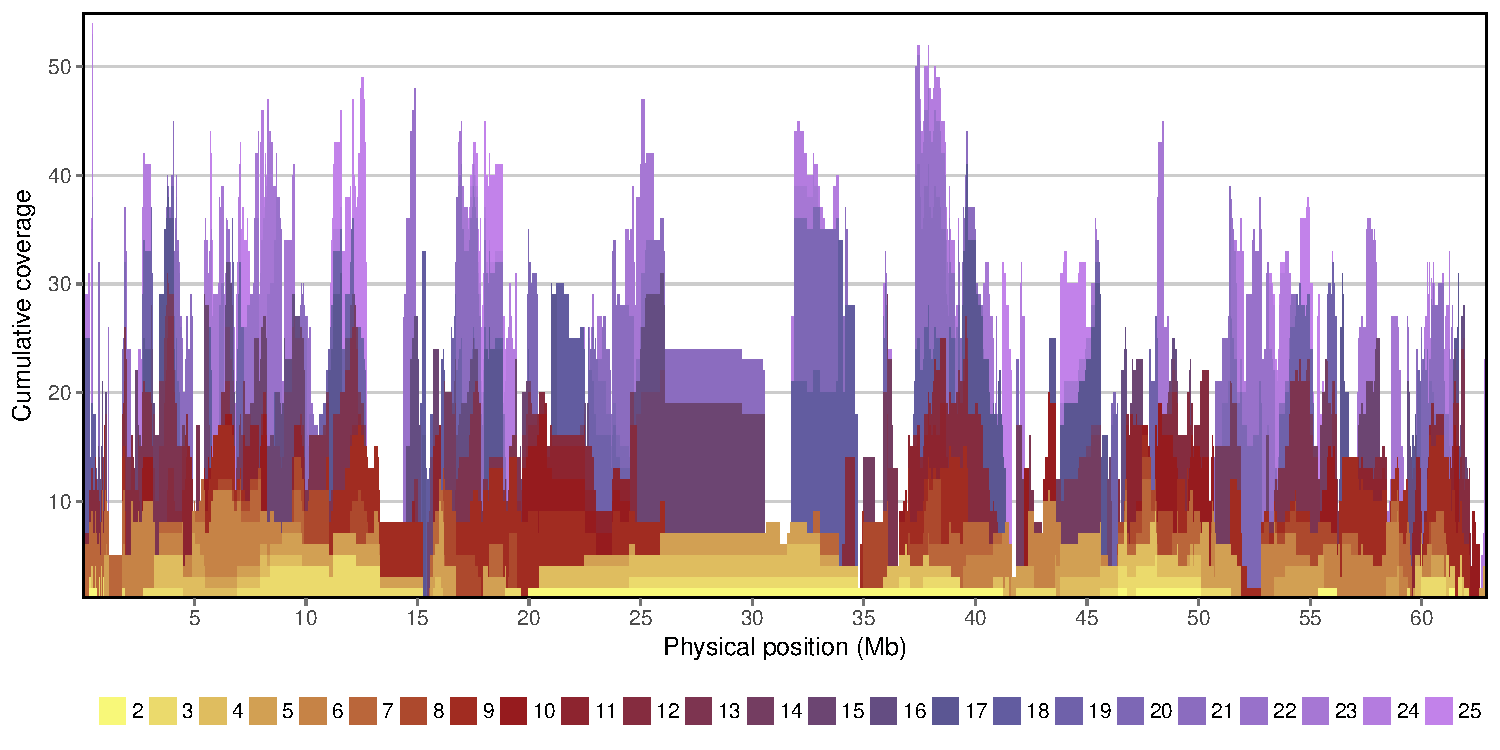
\includegraphics[width=\textwidth]{./img/ch3/phase_fk_coverage_example}
\Caption{Cumulative coverage of shared haplotypes along the chromosome}
{The cumulative coverage (\%) of a randomly chosen individual is illustrated.
All rare alleles (\fk{[2,25]}) which this individual shared with any other individual in the sample (${N=\num{2500}}$) were found and the \gls{dgt} was applied to detect segment breakpoints.
The set of retained unique segments was then stacked (lowest \fk{} variants at the bottom) to illustrate the cumulative coverage.
Segments are colour-coded by the frequency of the focal allele (\fk{}) around a segment was detected.}
{fig:phase_fk_coverage_example}
\end{figure}
